\documentclass[11pt]{article}

\usepackage[T1]{fontenc}
\usepackage[utf8]{inputenc}
\usepackage{lmodern}
\usepackage[a4paper,margin=1in]{geometry}
\usepackage{amsmath,amssymb,amsthm,mathtools}
\usepackage{float}
\usepackage{enumitem}
\usepackage{booktabs}
\usepackage{xcolor}
\usepackage{tikz}
\usepackage{hyperref}
\usetikzlibrary{arrows.meta,positioning,calc,fit,backgrounds}

\hypersetup{colorlinks=true,linkcolor=blue!70!black,citecolor=blue!70!black,urlcolor=blue!70!black}

% ── Theorem environments ──────────────────────────────────────────────────────
\newtheorem{theorem}{Theorem}[section]
\newtheorem{proposition}[theorem]{Proposition}
\newtheorem{lemma}[theorem]{Lemma}
\newtheorem{corollary}[theorem]{Corollary}
\theoremstyle{definition}
\newtheorem{definition}[theorem]{Definition}
\newtheorem{example}[theorem]{Example}
\theoremstyle{remark}
\newtheorem{remark}[theorem]{Remark}

% ── Macros (shared with paper.tex) ─────────────────────────────────────────────
\newcommand{\UDG}{\operatorname{UDG}}
\newcommand{\MWIS}{\mathrm{MWIS}}
\newcommand{\indep}{\alpha}
\newcommand{\R}{\mathbb{R}}
\newcommand{\tw}{\mathrm{tw}}
\newfloat{algorithm}{htbp}{loa}
\floatname{algorithm}{Algorithm}
\newcommand{\Comment}[1]{\hfill\textit{\footnotesize\textcolor{gray}{// #1}}}

\tikzset{
  v/.style={circle,draw,thick,minimum size=7mm,inner sep=0pt,font=\scriptsize},
  sep/.style={circle,draw,thick,fill=orange!35,minimum size=7mm,inner sep=0pt,font=\scriptsize},
  c1/.style={fill=red!28}, c2/.style={fill=blue!22}, c3/.style={fill=yellow!55},
}

\title{\textbf{A Decomposition Layer for Scaling Beyond the Atom Wall}\\[0.4em]
\large Block / tree-decomposition compilation of graph coloring to neutral-atom hardware}
\author{Research Draft --- companion to the main paper}
\date{\today}

\begin{document}
\maketitle

\begin{abstract}
The gadgetized reduction of $k$-coloring to unit-disk maximum-weight independent
set (MWIS) is exact, but its atom count grows as $O((nk)^2)$, so a few-hundred-atom
device caps the original graph at a handful of vertices. This note adds a
\emph{decomposition layer} in front of the reduction. Instead of compiling the
whole graph at once, we split it along small separators, encode one piece at a
time with its boundary fixed by precoloring constraints, solve each piece on the
device, and stitch the partial colorings classically. The peak hardware size then
depends on the \emph{width} $w$ of the decomposition --- the size of the largest
piece --- rather than on $n$:
\[
   |V(A)|_{\mathrm{peak}} \;=\; O\big((wk)^2\big).
\]
For graph classes of bounded width this is constant in $n$, so arbitrarily large
graphs become feasible; for general graphs it trades the device-size wall for a
classical cost of $O(k^{b})$ device solves per piece, where $b$ is the separator
size. We prove correctness for clique-separator decomposition (where stitching is
free) and state the general tree-decomposition dynamic program, give the atom-count
theorem, and finish with fully worked examples.
\end{abstract}

\tableofcontents

% =============================================================================
\section{Idea: decouple device size from $n$}
% =============================================================================

Recall from the main paper that compiling a coloring instance $(G,k)$ produces a
unit-disk MWIS instance $A$ with $nk \le |V(A)| = O((nk)^2)$ atoms, and that the
binding hardware constraint is the atom count $N_{\max}$. The quadratic growth is
the wall.

The decomposition layer rests on a classical fact: \emph{coloring is local}. Every
constraint of $G$ is a single edge, and edges do not span the whole graph --- they
live inside small neighborhoods. If we can carve $G$ into overlapping pieces so
that every edge sits inside some piece, we can color the pieces one at a time and
glue the results, provided the pieces agree on the vertices they share. The device
never holds more than one piece, so its size is governed by the \emph{largest
piece}, not by $G$.

\begin{center}
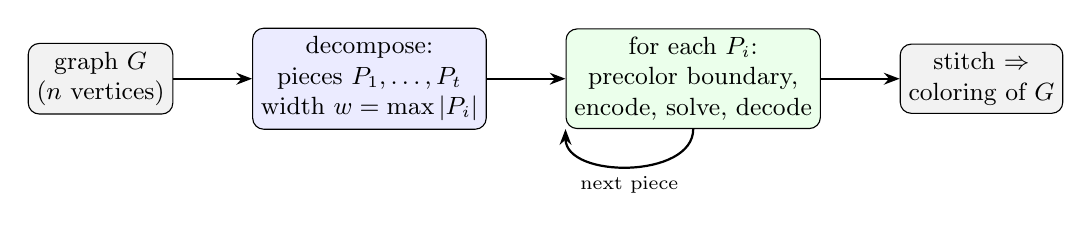
\begin{tikzpicture}[font=\small,node distance=7mm,
  b/.style={rectangle,draw,rounded corners,minimum height=8mm,align=center,inner sep=3pt},
  ar/.style={-{Stealth[length=2mm]},thick}]
  \node[b,fill=gray!10] (G) {graph $G$\\ ($n$ vertices)};
  \node[b,fill=blue!8,right=10mm of G] (dec) {decompose:\\ pieces $P_1,\dots,P_t$\\ width $w=\max|P_i|$};
  \node[b,fill=green!8,right=10mm of dec] (loop) {for each $P_i$:\\ precolor boundary,\\ encode, solve, decode};
  \node[b,fill=gray!10,right=10mm of loop] (out) {stitch $\Rightarrow$\\ coloring of $G$};
  \draw[ar] (G)--(dec); \draw[ar] (dec)--(loop); \draw[ar] (loop)--(out);
  \draw[ar] (loop.south) to[out=-90,in=-90] node[below,font=\scriptsize]{next piece} (loop.south west);
\end{tikzpicture}
\end{center}

The peak device size is $O((wk)^2)$ with $w$ the largest piece, so the entire
research question ``how large a graph can we handle?'' is re-parameterised from $n$
to $w$.

% =============================================================================
\section{Preliminaries: separators, blocks, and width}
% =============================================================================

\begin{definition}[Separator]
A vertex set $S\subseteq V$ is a \emph{separator} of a connected graph $G$ if
$G\setminus S$ has at least two connected components. $S$ is a \emph{clique
separator} if $G[S]$ is complete.
\end{definition}

\begin{definition}[Pieces of a separator]
Let $S$ separate $G$ into components $C_1,\dots,C_p$ of $G\setminus S$. The
\emph{pieces} are the induced subgraphs $G_j = G[S\cup C_j]$. Every piece contains
all of $S$; the pieces overlap exactly on $S$, and every edge of $G$ lies inside
some piece (an edge is either within $S$, or has an endpoint in some $C_j$ and
hence both endpoints in $G_j$).
\end{definition}

\begin{definition}[Tree decomposition and width~\cite{RobertsonSeymour1986}]
A \emph{tree decomposition} of $G$ is a tree $T$ whose nodes carry vertex sets
(\emph{bags}) $B_x\subseteq V$ such that (i) every vertex lies in some bag, (ii)
for every edge $\{u,v\}$ some bag contains both $u$ and $v$, and (iii) for every
vertex $v$ the bags containing $v$ form a connected subtree. The \emph{width} is
$\max_x |B_x|-1$, and the \emph{treewidth} $\tw(G)$ is the minimum width over all
tree decompositions.
\end{definition}

Throughout, the \emph{decomposition width} $w$ is the size of the largest piece
(clique-separator decomposition) or the largest bag (tree decomposition); these are
the quantities that will replace $n$ in the atom budget.

% =============================================================================
\section{Clique-separator decomposition: free stitching}
\label{sec:clique}
% =============================================================================

The cleanest case is when $G$ can be split along clique separators down to
\emph{atoms} (pieces with no further clique separator), as in the classical
decomposition of Dirac and Tarjan~\cite{Dirac1961,Tarjan1985}.

\begin{theorem}[Clique separators reduce coloring to pieces]
\label{thm:cliquesep}
Let $S$ be a clique separator of $G$ with pieces $G_1,\dots,G_p$. Then $G$ is
$k$-colorable if and only if every piece $G_j$ is $k$-colorable. Consequently, by
recursion, $\chi(G)=\max_j \chi(\mathrm{atom}_j)$ over the atoms of the
clique-separator decomposition.
\end{theorem}

\begin{proof}
($\Rightarrow$) A proper $k$-coloring of $G$ restricts to a proper $k$-coloring of
each induced subgraph $G_j$.

($\Leftarrow$) We glue two pieces at a time; recursion over the decomposition tree
finishes the argument. Suppose $G_1$ and $G_2$ share the clique separator $S$ and
each has a proper $k$-coloring, $c_1$ and $c_2$. Because $S$ is a clique, $c_1$ and
$c_2$ each assign $|S|$ \emph{distinct} colors to $S$; both are injections
$S\to\{1,\dots,k\}$, so there is a permutation $\pi$ of $\{1,\dots,k\}$ with
$\pi\circ(c_2|_S)=c_1|_S$ (match the two equal-size color images and extend $\pi$
arbitrarily on the remaining $k-|S|$ colors). Since recoloring by a permutation
preserves properness, $\pi\circ c_2$ is a proper $k$-coloring of $G_2$ that
\emph{agrees with $c_1$ on $S$}. The two now-consistent colorings combine into a
proper coloring of $G_1\cup G_2$: every edge lies in $G_1$ or $G_2$ and is properly
colored there, and the shared vertices $S$ carry one agreed color. (We use $k\ge
|S|$, which holds because $k\ge\chi(G_2)\ge\omega(G_2)\ge|S|$.)
\end{proof}

\begin{remark}[Why clique separators are ``free'']
The permutation argument needs \emph{no enumeration}: any two proper colorings of a
clique differ only by relabeling colors, so we can always realign a freshly solved
piece to its already-colored neighbor in $O(k)$ time. There is no $k^{|S|}$
branching. This is exactly why clique-separator decomposition is the preferred
front-end whenever it applies.
\end{remark}

% =============================================================================
\section{Per-piece encoding by boundary precoloring}
\label{sec:precolor}
% =============================================================================

When we solve a piece $G_i$, the vertices it shares with already-solved
neighbors --- its \emph{boundary} $B\subseteq V(G_i)$ --- already have fixed colors
$\beta:B\to\{1,\dots,k\}$. We bake $\beta$ into the Stage-1 reduction.

\begin{definition}[Boundary-precolored color-choice graph]
\label{def:precolorG}
Given a piece $G_i=(V_i,E_i)$, a boundary $B\subseteq V_i$, and a proper partial
coloring $\beta:B\to\{1,\dots,k\}$, define $G_i'(\beta)$ as the color-choice graph
of $(G_i,k)$ with one change: each boundary vertex $v\in B$ keeps \emph{only} its
single slot $(v,\beta(v))$ (its other $k-1$ slots and its choice clique are
deleted). Interior vertices $v\in V_i\setminus B$ keep all $k$ slots and their
choice clique as usual. Conflict edges are kept among all surviving slots.
\end{definition}

This is precisely the effect of the language's \texttt{precolor} restriction
applied to the boundary, and it shrinks the encoding: the logical-atom count drops
to
\[
   |V(G_i'(\beta))| \;=\; k\,(|V_i|-|B|) \;+\; |B| \;\le\; k\,|V_i|.
\]

\begin{proposition}[Exactness of the precolored encoding]
\label{prop:precolorexact}
$\indep\big(G_i'(\beta)\big) = |V_i|$ if and only if $G_i$ has a proper
$k$-coloring extending $\beta$. Moreover, every independent set of size $|V_i|$
decodes (one chosen slot per vertex) to such an extension.
\end{proposition}

\begin{proof}
This is the Stage-1 exactness theorem of the main paper with some slots pinned.
Any independent set takes at most one slot per vertex (the surviving choice
cliques on interior vertices; a single available slot on boundary vertices), so
its size is at most $|V_i|$, with equality iff exactly one slot per vertex is
chosen. The boundary slots $(v,\beta(v))$ are forced choices; they are mutually
non-adjacent because $\beta$ is proper, so they never block each other. A size-$|V_i|$
set therefore picks $\beta$ on $B$ and one color per interior vertex, and the
conflict edges guarantee adjacent vertices differ --- i.e.\ a proper coloring
extending $\beta$. The converse maps such a coloring to the corresponding slots,
which form an independent set of size $|V_i|$.
\end{proof}

Each piece is then gadgetized and solved exactly as in the main paper; only the
input graph $G_i'(\beta)$ is smaller and partly pinned.

% =============================================================================
\section{The general case: tree-decomposition dynamic program}
\label{sec:treedp}
% =============================================================================

Not every graph has helpful clique separators. The general tool is a tree
decomposition of width $w=\tw(G)$, processed by the standard dynamic program for
coloring on bounded treewidth~\cite{ArnborgProskurowski1989}. Here the separators
(adjacent-bag intersections) need not be cliques, so we cannot realign by a single
permutation; instead we enumerate the compatible boundary colorings.

\begin{definition}[Boundary table]
For a bag $B_x$ with separator $S_x=B_x\cap B_{\mathrm{parent}(x)}$, the
\emph{boundary table} $\mathcal{T}_x$ is the set of proper colorings $\beta$ of
$S_x$ that extend to a proper coloring of the subgraph induced by the subtree
rooted at $x$. There are at most $k^{|S_x|}\le k^{w+1}$ candidate $\beta$.
\end{definition}

\begin{proposition}[Per-bag device subproblem]
\label{prop:bagdp}
Processing the tree from the leaves up, $\beta\in\mathcal{T}_x$ if and only if, for
the colorings of the child separators already found compatible, the bag $B_x$ with
its separator precolored by $\beta$ admits a proper completion. Each such test is
one instance of Proposition~\ref{prop:precolorexact} on $G[B_x]$, i.e.\ one
device solve of an MWIS instance with $\le wk$ logical atoms. A nonempty table at
the root certifies $k$-colorability, and a top-down pass selects one compatible
$\beta$ per bag, yielding a global proper coloring.
\end{proposition}

\noindent This is the classical FPT-in-treewidth algorithm with each local
feasibility test delegated to the neutral-atom MWIS solver. The number of device
solves is $O(n\,k^{w+1})$ in the worst case --- the price of general (non-clique)
separators --- while the \emph{peak device size} stays $O((wk)^2)$.

% =============================================================================
\section{The decomposition-aware pipeline}
\label{sec:pipeline}
% =============================================================================

\begin{algorithm}[h]
\caption{Decomposition-aware coloring-to-neutral-atom compiler}
\label{alg:dec}
\rule{\linewidth}{0.4pt}\vspace{-2pt}
\begin{flushleft}
\textbf{Input:} graph $G=(V,E)$, palette $k$, hardware budget $N_{\max}$.\\
\textbf{Output:} proper $k$-coloring of $G$, or ``not $k$-colorable''.
\end{flushleft}
\vspace{-4pt}\rule{\linewidth}{0.4pt}
\begin{enumerate}[leftmargin=2.4em,itemsep=1pt,label=\arabic*.]
\item \textbf{Preprocess:} iteratively remove vertices of degree $<k$ (the
      $k$-core); they are colored greedily at the very end. \Comment{shrinks $G$}
\item \textbf{Decompose:} compute a clique-separator decomposition into atoms
      \cite{Tarjan1985}; for atoms still too large, refine with a tree
      decomposition of width $w$ \cite{Bodlaender1996}. Let $P_1,\dots,P_t$ be the
      pieces, ordered by a rooted decomposition tree. \Comment{$w=\max_i|P_i|$}
\item \textbf{Check budget:} require $O((wk)^2)\le N_{\max}$; else refine further
      or report infeasible. \Comment{peak size depends on $w$, not $n$}
\item \textbf{For each piece $P_i$ in tree order:}
      \begin{enumerate}[leftmargin=1.6em,label=(\alph*),itemsep=0pt]
        \item read the boundary coloring $\beta$ from already-solved neighbors
              (clique separator: a single $\beta$; general: iterate over the
              boundary table $\mathcal{T}$);
        \item build $G_i'(\beta)$ (Def.~\ref{def:precolorG}), gadgetize to a UDG
              MWIS instance, solve on the device, decode
              (Prop.~\ref{prop:precolorexact});
        \item if no size-$|P_i|$ set exists for any $\beta$, report ``not
              $k$-colorable''; else record the piece's coloring (clique case:
              realign by the permutation of Thm.~\ref{thm:cliquesep}).
      \end{enumerate}
\item \textbf{Stitch:} the recorded colorings agree on shared vertices by
      construction; output their union, then color the peeled degree-$<k$ vertices.
\end{enumerate}
\vspace{-4pt}\rule{\linewidth}{0.4pt}
\end{algorithm}

\begin{theorem}[Soundness of stitching]
\label{thm:stitch}
If Algorithm~\ref{alg:dec} records, for every piece $P_i$, a proper $k$-coloring of
$P_i$ such that any two pieces agree on their shared vertices, then the union is a
proper $k$-coloring of $G$.
\end{theorem}

\begin{proof}
Take any edge $\{u,v\}\in E$. Because every edge lies inside some piece (clique
case) or some bag (tree-decomposition case), there is a piece $P_i$ with
$u,v\in P_i$. The recorded coloring of $P_i$ is proper, so $c(u)\ne c(v)$. The
assignment is well defined because pieces agree on shared vertices. Hence every
edge is properly colored. The peeled vertices have degree $<k$ at removal time, so
each has a free color when reinserted in reverse order.
\end{proof}

% =============================================================================
\section{The scaling result}
\label{sec:scaling}
% =============================================================================

\begin{theorem}[Peak atom count]
\label{thm:peak}
Let $G$ admit a decomposition of width $w$ into $t$ pieces with maximum separator
size $b$. Algorithm~\ref{alg:dec} solves $k$-coloring with
\[
   |V(A)|_{\mathrm{peak}} \;=\; O\big((wk)^2\big)\ \text{atoms on the device at any one time},
\]
using at most $t$ device solves when all separators are cliques
(Thm.~\ref{thm:cliquesep}), and $O(t\,k^{\,b})$ device solves in general
(Prop.~\ref{prop:bagdp}). The classical work outside the device is
$\mathrm{poly}(n)$ per solve.
\end{theorem}

\begin{proof}
At any moment the device holds the gadgetization of a single $G_i'(\beta)$, which
has at most $wk$ logical atoms (Def.~\ref{def:precolorG}) and hence $O((wk)^2)$
atoms after gadgetization (main-paper atom bound). The solve counts are those of
Theorem~\ref{thm:cliquesep} (one $\beta$ per piece) and
Proposition~\ref{prop:bagdp} ($\le k^{b}$ boundary colorings per piece). Building
each $G_i'(\beta)$, gadgetizing, decoding, and stitching are all polynomial.
\end{proof}

The wall has moved from $n$ to $w$. Three regimes make the consequence concrete
(taking $k=3$, and a worst-case atom constant $|V(A)|\approx (wk)^2$):

\begin{table}[h]
\centering
\begin{tabular}{@{}lll l@{}}
\toprule
Graph class & width $w$ & peak atoms $O((wk)^2)$ & consequence \\
\midrule
trees, $k$-degenerate cores emptied & $1$ & $O(k^2)\approx 9$ & any $n$, trivially \\
series--parallel / outerplanar & $\le 2$ & $\approx 36$ & any $n$ \\
bounded treewidth (fixed $w$) & $O(1)$ & $O(k^2)$ const. & \textbf{any $n$ at constant device size} \\
``sparse with small dense pockets'' & small const.\ blocks & const. & any $n$ \\
planar (general) & $\Theta(\sqrt n)$ & $\Theta(n k^2)$ & \emph{linear} in $n$ (was quadratic) \\
arbitrary dense & $\Theta(n)$ & $\Theta((nk)^2)$ & no improvement \\
\bottomrule
\end{tabular}
\caption{Peak device size is set by the decomposition width $w$, not by $n$. For
bounded-width classes the device size is constant in $n$.}
\label{tab:regimes}
\end{table}

\begin{corollary}[Hundreds of vertices, concretely]
\label{cor:hundreds}
A graph whose pieces all have $\le w$ vertices is solvable with peak device size
$O((wk)^2)$ regardless of $n$. For instance, with $w=15$ and $k=4$ the peak is
$\approx (60)^2 = 3600$ logical atoms before gadgetization and a few hundred atoms
after a crossing-minimized layout of each small piece --- well within a
$1000$-atom array --- so a graph of \emph{several hundred} vertices is colored as a
sequence of small device solves. With $w=O(1)$ (e.g.\ a chain of small blocks) the
peak is a fixed handful of atoms and $n$ is unbounded; see
Example~\ref{ex:chain}.
\end{corollary}

\begin{remark}[Cost honesty]
The improvement is real but not free. (i) For non-clique separators the
$O(k^{b})$ factor is exponential in the separator size $b$, so the method is
practical only when separators are small (clique separators give $b$ effectively
$0$; bounded treewidth gives $b\le w+1=O(1)$). (ii) Finding a good decomposition is
itself work: clique-separator atoms are computable in polynomial
time~\cite{Tarjan1985}, and an optimal-width tree decomposition is fixed-parameter
tractable~\cite{Bodlaender1996} with good heuristics in practice. (iii) Dense
graphs have $w=\Theta(n)$ and gain nothing --- decomposition helps exactly the
structured, sparse instances, which is where the rest of the pipeline already
lives.
\end{remark}

\begin{remark}[Toward the type system]
Decomposition turns compilation into a \emph{composition of certified sub-solves}.
Each piece carries a coloring decoded against the instance that produced it, and
the boundary precoloring is a constraint shared between adjacent pieces. A future
type system can track this directly: provenance of each partial coloring, the
\texttt{precolor} obligations linking neighbors, and a stitching rule whose
well-typedness witnesses Theorem~\ref{thm:stitch}. ``Reaching hundreds of
vertices'' and ``what does the type system buy us'' become the same question ---
compositional, certificate-carrying compilation.
\end{remark}

% =============================================================================
\section{Worked examples}
\label{sec:examples}
% =============================================================================

We finish with fully explicit examples, in the step-by-step style of the
companion examples document.

\subsection{Example A --- the bowtie: a single cut vertex}

\textbf{The graph.} Two triangles sharing one vertex $c$ (the \emph{bowtie}):
$\{\ell_1,\ell_2,c\}$ and $\{c,r_1,r_2\}$. Here $S=\{c\}$ is a clique separator of
size $1$ (a cut vertex), and the two pieces are the two triangles. $n=5$.

\begin{center}
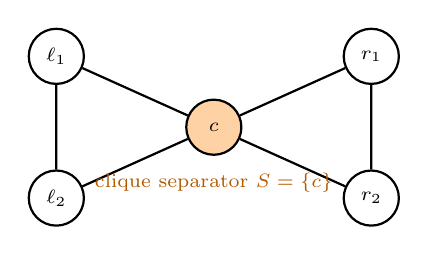
\begin{tikzpicture}[scale=1]
  \node[v] (l1) at (-2,0.9){$\ell_1$};
  \node[v] (l2) at (-2,-0.9){$\ell_2$};
  \node[sep] (c) at (0,0){$c$};
  \node[v] (r1) at (2,0.9){$r_1$};
  \node[v] (r2) at (2,-0.9){$r_2$};
  \draw[thick] (l1)--(l2)--(c)--(l1);
  \draw[thick] (r1)--(r2)--(c)--(r1);
  \node[font=\scriptsize,orange!70!black] at (0,-0.7){clique separator $S=\{c\}$};
\end{tikzpicture}
\end{center}

\paragraph{Step 1 --- decompose.} Cut at $c$: piece $P_1=\{\ell_1,\ell_2,c\}$
(a triangle), piece $P_2=\{c,r_1,r_2\}$ (a triangle). Width $w=3$. Each triangle
needs $k=3$ (Thm.~\ref{thm:cliquesep} gives $\chi=\max(3,3)=3$).

\paragraph{Step 2 --- solve $P_1$ (no boundary yet).} Build the color-choice graph
of the triangle with $k=3$ and solve, exactly as in the companion document: the
MWIS picks one slot per vertex in distinct rows, e.g.
\[
   c\mapsto 1,\quad \ell_1\mapsto 2,\quad \ell_2\mapsto 3.
\]
Record this. Note the device only ever sees a $3$-vertex piece
($|V(G_1')|=nk=9$ logical atoms), not the whole bowtie.

\paragraph{Step 3 --- solve $P_2$ with boundary precolored.} The boundary is
$B=\{c\}$ with $\beta(c)=1$ (inherited from $P_1$). By
Definition~\ref{def:precolorG}, $c$ keeps only its slot $(c,1)$; $r_1,r_2$ keep all
three slots. Solving $G_2'(\beta)$ (Prop.~\ref{prop:precolorexact}) yields a proper
extension, e.g.
\[
   c\mapsto 1\ (\text{fixed}),\quad r_1\mapsto 2,\quad r_2\mapsto 3.
\]

\begin{center}
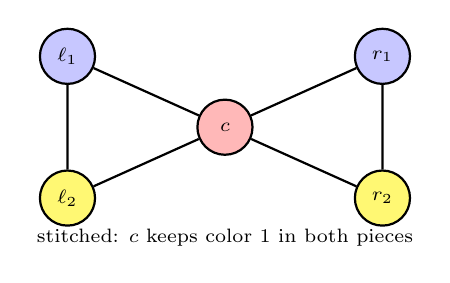
\begin{tikzpicture}[scale=1]
  \node[v,c2] (l1) at (-2,0.9){$\ell_1$};
  \node[v,c3] (l2) at (-2,-0.9){$\ell_2$};
  \node[v,c1] (c) at (0,0){$c$};
  \node[v,c2] (r1) at (2,0.9){$r_1$};
  \node[v,c3] (r2) at (2,-0.9){$r_2$};
  \draw[thick] (l1)--(l2)--(c)--(l1);
  \draw[thick] (r1)--(r2)--(c)--(r1);
  \node[font=\scriptsize] at (0,-1.4){stitched: $c$ keeps color $1$ in both pieces};
\end{tikzpicture}
\end{center}

\paragraph{Step 4 --- stitch.} Both pieces agree on $c$ (color $1$) by
construction, so their union is a proper $3$-coloring of the bowtie
(Thm.~\ref{thm:stitch}). \textbf{Peak device size:} one triangle ($9$ logical
atoms), versus $15$ for the monolithic bowtie --- and crucially the peak is
independent of how many triangles we attach, which is the next example.

\subsection{Example B --- a chain of triangles: $n\to\infty$ at constant device size}
\label{ex:chain}

\textbf{The graph.} Glue $t$ triangles in a line, each sharing one cut vertex with
the next: vertices $v_0,v_1,\dots,v_{2t}$, with triangles
$\{v_{2j},v_{2j+1},v_{2j+2}\}$ for $j=0,\dots,t-1$. Then $n=2t+1$ grows without
bound, but every piece is a triangle, so $w=3$ \emph{for all $t$}.

\begin{center}
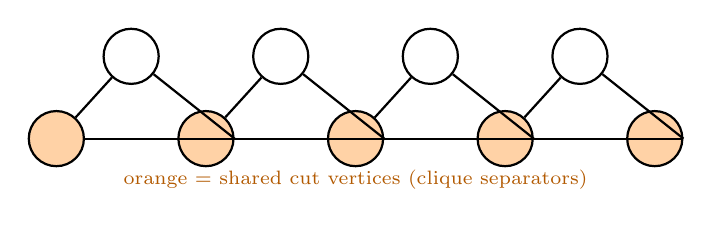
\begin{tikzpicture}[scale=0.95]
  % chain of 4 triangles sharing apex cut vertices on a line
  \foreach \j in {0,1,2,3}{
    \pgfmathsetmacro\xa{2*\j}
    \pgfmathsetmacro\xb{2*\j+2}
    \pgfmathsetmacro\xm{2*\j+1}
    \node[sep] (b\j) at (\xa,0){};
    \node[v]   (t\j) at (\xm,1.1){};
    \draw[thick] (b\j) -- (t\j);
  }
  \node[sep] (b4) at (8,0){};
  \foreach \j in {0,1,2,3}{
    \pgfmathsetmacro\next{\j+1}
    \draw[thick] (b\j) -- (b\next);
    \draw[thick] (t\j) -- (b\next);
  }
  \node[font=\scriptsize,orange!70!black] at (4,-0.55){orange = shared cut vertices (clique separators)};
\end{tikzpicture}
\end{center}

\paragraph{Solve.} Process triangles left to right. The first is solved freely
($3$ colors). Each subsequent triangle shares exactly one already-colored vertex;
precolor it (boundary size $1$) and solve, then realign by the color permutation of
Theorem~\ref{thm:cliquesep} if needed. Every device solve is a single triangle:
$|V(G_i'(\beta))| \le 9$ logical atoms.

\paragraph{The point.} By Theorem~\ref{thm:peak}, the peak device size is
$O((3k)^2)$ --- a fixed handful of atoms --- \emph{for every $t$}. A $201$-vertex
chain ($t=100$) is colored by $100$ tiny sequential solves; a $2001$-vertex chain
the same way. The atom wall has been removed for this class entirely: $n$ is
unbounded at constant hardware size. This is the concrete sense in which hundreds
(or thousands) of vertices are reachable.

\subsection{Example C --- a non-clique separator: paying the $k^{b}$ price}

\textbf{The graph.} Two squares glued along a non-adjacent vertex pair. Let
$P_1$ be the $4$-cycle $a\,x\,b\,y$ and $P_2$ the $4$-cycle $a\,p\,b\,q$, sharing
$S=\{a,b\}$, with $a,b$ \emph{not} adjacent. Now $S$ is a separator but \emph{not}
a clique, so the free permutation trick does not apply --- we must enumerate
boundary colorings.

\begin{center}
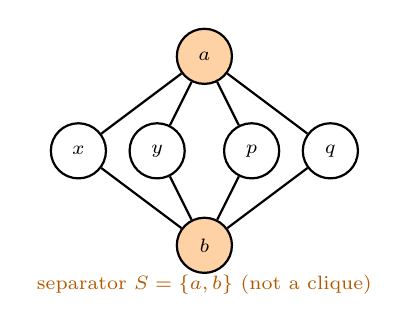
\begin{tikzpicture}[scale=1]
  \node[sep] (a) at (0,1.2){$a$};
  \node[sep] (b) at (0,-1.2){$b$};
  \node[v] (x) at (-1.6,0){$x$};
  \node[v] (y) at (-0.6,0){$y$};
  \node[v] (p) at (0.6,0){$p$};
  \node[v] (q) at (1.6,0){$q$};
  \draw[thick] (a)--(x)--(b)--(y)--(a);
  \draw[thick] (a)--(p)--(b)--(q)--(a);
  \node[font=\scriptsize,orange!70!black] at (0,-1.7){separator $S=\{a,b\}$ (not a clique)};
\end{tikzpicture}
\end{center}

\paragraph{Solve with $k=2$.} The boundary table over $S=\{a,b\}$ has at most
$k^{|S|}=2^2=4$ candidates: $(a,b)\in\{(1,1),(1,2),(2,1),(2,2)\}$. For each, run the
precolored solve on each square:
\begin{itemize}[leftmargin=1.4em,itemsep=1pt]
  \item $\beta=(a{=}1,b{=}2)$: each square completes ($x,p\mapsto$ \dots), compatible
        on both sides --- a global $2$-coloring exists. \checkmark
  \item $\beta=(a{=}1,b{=}1)$: in $P_1$, vertex $x$ is adjacent to both $a$ and $b$,
        now both colored $1$, so $x$ needs a second color --- fine for $k=2$
        ($x\mapsto2$); but $y$ likewise must be $2$, and $a,b$ equal is allowed since
        $a,b$ non-adjacent. This $\beta$ also completes. \checkmark
\end{itemize}
We keep any $\beta$ that completes on \emph{both} pieces and stitch. The extra cost
versus the clique case is the up-to-$4$ boundary colorings we had to try ---
exactly the $O(k^{b})$ factor of Theorem~\ref{thm:peak} with $b=|S|=2$. Had $S$
been a clique (an edge $a\!-\!b$), only the $\beta$ with $a\ne b$ would survive and
no enumeration would be needed.

\paragraph{Lesson.} Small separators keep the $k^{b}$ factor tiny; clique
separators make it vanish. This is why the front-end prefers clique-separator atoms
and, failing that, low-treewidth bags --- precisely the structure that also keeps
the per-piece encoding small.

% =============================================================================
\bibliographystyle{plain}
\bibliography{references}
% =============================================================================

\end{document}
